\chapter{Tests and Benchmarks}\label{chap:test}
\begin{mybox}
After the presentation of the main theoretical contents, we are going to show in this chapter some results of the implementation:

\begin{itemize}
    \item Comparison of PermReach, ASPReach which were introduced in Chapter~\ref{chap:refinement} with several state-of-the-art model checkers: exhaustive reachability analyzers (Mole, NuSMV and ASP solver without optimization), Pint on their scalability (biggest tractable model size), efficiency (runtime) and precision (global conclusiveness)
    \item As there is no model revision technique based on reachability in the literature, we are going to show the performance of CRAC and M2RIT in Chapter~\ref{chap:modelInference} on random examples of different sizes.
\end{itemize}
\end{mybox}

In Chapter~\ref{chap:refinement}, we have illustrated the concepts of the new modeling framework ABAN and several related definitions which describe the reachability problem under this framework.
Afterwards, we have shown the theoretical effectiveness and correctness of our reachability analyzers PermReach and ASPReach. 
To ensure their capacity, we use small models to verify the correctness, \textit{i.e.} PermReach and ASPReach obtain the same result as other model checkers.
Then we apply all the analyzers on a series of models with increasing sizes to obtain the limit of the capacity of each analyzer.
These tests show our analyzers can be applied to models with more than $1000$ automata while traditional ones fail at models with $50$ automata.

As for CRAC and M2RIT, CRAC uses reachability properties and \textit{continuous} time-series data while M2RIT uses reachability properties and \textit{discretized} time-series data.


\section{Comparison of Reachability Analyzers}\label{sec:compReachAnalyzers}
In this section, we evaluate the reachability analyzers through tests on computing power, conclusiveness and results on random examples.
The competitors are
\begin{itemize}
    \item traditional model checkers Mole\footnote{\url{http://www.lsv.fr/~schwoon/tools/mole}} and NuSMV\footnote{\url{http://nusmv.fbk.eu}}, pure ASP solver~\cite{abdallah2015exhaustive}
    \item pure static analyzer Pint~\cite{pauleve2017reduction}
    \item our hybrid analyzers PermReach and ASPReach
\end{itemize}

All tests were run on an Intel Core i7-3770 CPU, \@3.4GHz with 8GB RAM computer.

\subsection{Performance on Computing Power}
To evaluate the scalability in \textit{in silico} networks, we take T-cell Receptor model (TCR)~\cite{saez2007logical} and epidermal growth factor receptor model (EGFR)~\cite{samaga2009logic} as examples, with the former one containing $95$ automata and $206$ transitions and the latter one containing $104$ automata and $389$ transitions respectively. 

These models are originally Boolean networks.
According to the approach in Appendix~\ref{appendix:trans}, BNs are transformed into ABANs. 
Here, we ran the same test as in~\cite{folschette2015}. In the TCR model, we take $3$ automata as input (\texttt{cd4 cd28 tcrlig}), vary exhaustively their initial states combinations ($2^3$) and finally take the reachability of states of $5$ automata (\texttt{sre ap1 nfkb nfat sigmab}) as output. 
Similarly we carried a bigger test on EGFR model with $13$ automata %\footnote{\texttt{erbb1 erbb2 erbb3 erbb4 bir btc egf epr nrg1a nrg1b nrg2b nrg4 tgfa}}
as input and $12$ automata %\footnote{\texttt{elk1 creb ap1 hsp27 actin\_reorg cmyc pro\_apoptotic p70s6\_2 pkc stat1 stat3 stat5}}
as output.
We first tested the performance of traditional model checkers and pure ASP approach which have the biggest theoretical complexities. 
For traditional model checkers, Mole turns out to be memory-out for $6$ in $12$ outputs, and all memory-out for NuSMV in model EGFR. 

Ben-Abdallah \textit{et al.}~\cite{abdallah2015exhaustive} have implemented reachability analyzer using pure ASP solver, showing it has a runtime of the same scale (See Appendix~\ref{chap:pureASP}).
Thanks to the efficiency of Clingo\footnote{\url{http://potassco.sourceforge.net/}}, pure ASP solver begins to fail at $80$ automata rather than $50$ which is the limit of traditional model checkers. 
But this computational capacity is still not enough as the number of automata in systems biology is usually in the scale of $10^3$ or bigger.

Due to the big state space, traditional model checkers and pure ASP method are not applicable but they can be used to validate non-exhaustive approaches on small examples.
The runtime results of Pint, PermReach and ASPReach are listed in Table~\ref{tab:results} on page~\pageref{tab:results}.
Pint runs faster than ASPReach in TCR test but slower in EGFR test because there are inconclusive instances which cost more the runtime.

\subsection{Performance on Conclusiveness}
To validate our approaches, we carried tests on a small example, $\lambda$-phage model~\cite{thieffry1995dynamical} to compare with an alternative reachability analyzer Pint~\cite{pauleve2012} implementing solely an analysis using LCG~\cite{pauleve2017reduction,folschette2015,pauleve2011}.
$\lambda$-phage is originally a multivalued model.
We compressed its multivalued variables to transform it into a Boolean model.
In this model with 4 automata and $12$ transitions (without taking consideration of the self-regulations),
PermReach and ASPReach show complete conclusiveness while Pint cannot (Figure~\ref{fig:LCG_lambdaPhage}). %able to figure out the reachability of $cro_1$ when $cI_1$ and $cII_1$ are in the initial state (Figure~\ref{fig:LCG_lambdaPhage}).
Pint cannot decide whether $cro_1$ is reachable or not, because it does not consider the order in the state sequence even though there exists a solution of length 3: $cII_0::cI_0::cro_0$ corresponding to the trajectory $\acm{cI_1}{cII_1}{cII_0}::\acm{cII_0}{cI_1}{cI_0}::\acm{cII_0,cI_0}{cro_0}{cro_0}$.
\begin{figure}[ht]
\centering
    \begin{tikzpicture}[aS]  
  	
  	\startl{cro_1};
  	\specl{above}{cro_1}{cII_0};
  	\link{cII_0}{cI_1};
  	\edl{cI_1};
  	\specl{below}{cro_1}{cI_0};
	\path (cI_0s) edge (cII_0);
    
    \end{tikzpicture}

    \caption[SLCG of $\lambda$-phage model]{An SLCG of $\lambda$-phage model, automaton $cI$ appears in both branches of the \textbf{AND gate}.
    Pint cannot decide the reachability of $cro_0$.}
    \label{fig:LCG_lambdaPhage}
\end{figure}

When dealing with more complex topology of SLCGs in term of branches, PermReach is not able to handle some of the special cases where multiple states of one automaton appear in different branches (Figure~\ref{fig:countexPerm}).
Theses cases are solvable by \mbox{ASPReach}.

\begin{figure}[ht]
    \centering
    \begin{tikzpicture}[aS]  
  	
	\startl{a_1};
	\specl{above}{a_1}{b_1};
	\specl{above}{b_1}{d_0};
	\edl{d_0};
	\link{b_1}{a_0};
 	\edl{a_0};
	\link{a_1}{c_1};
 	\link{c_1}{d_1};
 	\link{d_1}{c_0};
 	\edl{c_0};
 	\specl{below}{c_1}{e_0};
 	\edl{e_0};
    \end{tikzpicture}
    \caption[Counterexample of PermReach]{Counterexample of SLCG that cannot be solved by PermReach. The former counterexample shows PermReach is not fully inconclusive.}\label{fig:countexPerm}
\end{figure}

PermReach is not able to deal with the cases where multiple states of one automaton appear in the branches of one \textbf{AND gate} ($d_0$ and $d_1$ in this example).
There exists a consistent state sequence: $d_1::b_1::c_1::a_1$ corresponding to the trajectory $\acm{c_0}{d_0}{d_1}::\acm{d_0,a_0}{b_0}{b_1}::\acm{d_1,e_0}{c_0}{c_1}::\acm{b_1,c_1}{a_0}{a_1}$ which could be found by ASPReach.

The whole approach is implemented in Python3\footnote{Code and testing data available at \url{https://github.com/XinweiChai/reach_and_revision}}.
The call of ASP in Python is done by package \textit{pyasp}\footnote{\url{https://pypi.python.org/pypi/pyasp}}. 

In the TCR tests, our approach gives exactly the same result as Pint did. 
As for EGFR tests, ASPReach returned no inconclusive output.

\begin{table}[ht]
\centering
\begin{small}
    \begin{tabular}{|c|c|c|c|}
    \hline
     Model    &  \multicolumn{3}{c|}{$\lambda$-phage}\\
     \hline
     Inputs    & 4 & Outputs& 4\\%\multicolumn{3}{c|}{4}\\
     \hline
     Total tests&\multicolumn{3}{c|}{$2^4\times 4=64$}\\
     \hline
     Analyzer  &  Pint  &  \textbf{PermReach}   &\textbf{ASPReach}\\
     \hline
     Reachable & 36(56\%)& \multicolumn{2}{c|}{38(59\%)} \\
     \hline
     Unreachable&\multicolumn{3}{c|}{26(41\%)}\\
     \hline
     \textbf{Inconclusive} &\textcolor{red}{\textbf{2(3\%)}}&\multicolumn{2}{c|}{\textcolor{blue}{\textbf{0(0\%)}}}\\
     \hline
     Total time & \multicolumn{3}{c|}{$<1$s}\\
    \hline
     Model    &  \multicolumn{3}{c|}{TCR}\\
     \hline
     Inputs    & 3 & Outputs& 5\\
     \hline
     Total tests&\multicolumn{3}{c|}{$2^3\times 5=40$}\\
     \hline
     Analyzer  &  Pint  &  \textbf{PermReach}   &\textbf{ASPReach}\\
     \hline
     Reachable & \multicolumn{3}{c|}{16(40\%)} \\
     \hline
     Unreachable&\multicolumn{3}{c|}{24(60\%)} \\
     \hline
     \textbf{Inconclusive} &\multicolumn{3}{c|}{\textcolor{blue}{\textbf{0(0\%)}}} \\
     \hline
     Total time &  7s     &0.85s  &  40s        \\
    \hline
     Model    &  \multicolumn{3}{c|}{EGFR}\\
     \hline
     Inputs    & 13 & Outputs& 12\\
     \hline
     Total tests&\multicolumn{3}{c|}{$2^{13}\times 12=98,304$}\\
     \hline
     Analyzer  &  Pint  &  \textbf{PermReach}   &\textbf{ASPReach}\\
     \hline
     Reachable & 64,282(65.4\%)  & \multicolumn{2}{c|}{74,268(75.5\%)} \\
     \hline
     Unreachable&\multicolumn{3}{c|}{24,036(24.5\%)}\\
     \hline
     \textbf{Inconclusive} &\textcolor{red}{\textbf{9,986(10.1\%)}}&\multicolumn{2}{c|}{\textcolor{blue}{\textbf{0(0\%)}}}   \\
     \hline
     Total time & \textbf{9h50min}      & \textbf{15min31s}         & \textbf{3h46min} \\
     \hline
    \end{tabular}
\end{small}
    %\begin{tabular}{|c|c|c|c|}
    %\hline
    % Model    &  \multicolumn{3}{c|}{$\lambda$-phage}\\
    % \hline
    % Inputs    & \multicolumn{3}{c|}{4}\\
    % \hline
    % Outputs&\multicolumn{3}{c|}{4}\\
    % \hline
    % Total tests&\multicolumn{3}{c|}{$2^4\times 4=64$}\\
    % \hline
    % Analyzer  &  Pint  &  \textbf{PermReach}   &\textbf{ASPReach}\\
    % \hline
    % Reachable & 36(56\%)& \multicolumn{2}{c|}{38(59\%)} \\
    % \hline
    % Unreachable&\multicolumn{3}{c|}{26(41\%)}\\
    % \hline
    % \textbf{Inconclusive} &\textcolor{red}{\textbf{2(3\%)}}&\multicolumn{2}{c|}{\textcolor{blue}{\textbf{0(0\%)}}}\\
    % \hline
    % Total time & \multicolumn{3}{c|}{$<1$s}\\
    %\hline
    % Model    &  \multicolumn{3}{c|}{TCR}\\
    % \hline
    % Inputs    & \multicolumn{3}{c|}{3}\\
    % \hline
    % Outputs&\multicolumn{3}{c|}{5}\\
    % \hline
    % Total tests&\multicolumn{3}{c|}{$2^3\times 5=40$}\\
    % \hline
    % Analyzer  &  Pint  &  \textbf{PermReach}   &\textbf{ASPReach}\\
    % \hline
    % Reachable & \multicolumn{3}{c|}{16(40\%)} \\
    % \hline
    % Unreachable&\multicolumn{3}{c|}{24(60\%)} \\
    % \hline
    % \textbf{Inconclusive} &\multicolumn{3}{c|}{\textcolor{blue}{\textbf{0(0\%)}}} \\
    % \hline
    % Total time &  7s     &0.85s  &  40s        \\
    %\hline
    % Model    &  \multicolumn{3}{c|}{EGFR}\\
    % \hline
    % Inputs    & \multicolumn{3}{c|}{13}\\
    % \hline
    % Outputs&\multicolumn{3}{c|}{12}\\
    % \hline
    % Total tests&\multicolumn{3}{c|}{$2^{13}\times 12=98,304$}\\
    % \hline
    % Analyzer  &  Pint  &  \textbf{PermReach}   &\textbf{ASPReach}\\
    % \hline
    % Reachable & 64,282(65.4\%)  & \multicolumn{2}{c|}{74,268(75.5\%)} \\
    % \hline
    % Unreachable&\multicolumn{3}{c|}{24,036(24.5\%)}\\
    % \hline
    % \textbf{Inconclusive} &\textcolor{red}{\textbf{9,986(10.1\%)}}&\multicolumn{2}{c|}{\textcolor{blue}{\textbf{0(0\%)}}}   \\
    % \hline
    % Total time & \textbf{9h50min}      & \textbf{15min31s}         & \textbf{3h46min} \\
    % \hline
    %\end{tabular}
    
    %\begin{tabular}{|c|c|c|c|c|c|c|c|c|c|}
    %\hline
  	%Model	&\multicolumn{3}{c|}{$\lambda$-phage}	&	  \multicolumn{3}{c|}{TCR} & \multicolumn{3}{c|}{EGFR}  \\
    %\hline
    %Inputs&\multicolumn{3}{c|}{4}	&	  \multicolumn{3}{c|}{3} & \multicolumn{3}{c|}{13}\\
    %\hline
    %Outputs&\multicolumn{3}{c|}{4} &	  \multicolumn{3}{c|}{5} & \multicolumn{3}{c|}{12} \\
    %\hline
    %Total tests&\multicolumn{3}{c|}{$2^4\times 4=64$} & \multicolumn{3}{c|}{$2^3\times 5=40$} & \multicolumn{3}{c|}{$2^{13}\times 12=98,304$}\\
    %\hline
    %Analyzer  &  Pint  &  \textbf{PermReach}   &\textbf{ASPReach}    &  Pint  &  \textbf{PermReach}     &\textbf{ASPReach}   &  Pint  &  \textbf{PermReach}     &\textbf{ASPReach}             \\
    %\hline
    %Reachable    & 36(56\%)& 38(59\%)& 38(59\%)   &  \multicolumn{3}{c|}{16(40\%)}  & 64,282(65.4\%)  & \multicolumn{2}{c|}{74,268(75.5\%)}\\
    %\hline
    %\textbf{Inconclusive} & \textcolor{red}{\textbf{2(3\%)}}&\multicolumn{2}{c|}{\textcolor{blue}{\textbf{0(0\%)}}}& \multicolumn{3}{c|}{0(0\%)}    &\textcolor{red}{\textbf{9,986(10.1\%)}}&\multicolumn{2}{c|}{\textcolor{blue}{\textbf{0(0\%)}}}  \\
    %\hline
    %Unreachable     &  \multicolumn{3}{c|}{26(41\%)} &  \multicolumn{3}{c|}{24(60\%)} &\multicolumn{3}{c|}{24,036(24.5\%)}\\
    %\hline
    %Total time &  \multicolumn{3}{c|}{$<1$s}        &  7s     &0.85s  &  40s        & \textbf{9h50min}      & \textbf{15min31s}         & \textbf{3h46min}      \\
    %\hline
    %\end{tabular}
\caption[Comparison of different analyzers]{
Results of the tests on small ($\lambda$-phage) and large (TCR, EGFR) examples from literature. 
``Reachable'', ``Inconclusive'' and ``Unreachable'' give respectively the number of different results of reachability, while ``Total time'' depict the maximum time of the individual computations.}\label{tab:results}
\end{table}

As seen in Table~\ref{tab:results} on page \pageref{tab:results}, our approach can be more conclusive than Pint for ABANs.
Model-checkers using global search are perfectly conclusive for all tests (including $\lambda$-phage model) and memory-out on latter two tests so they are not listed in the table.
In the configuration of heuristics, we set a threshold for \textbf{OR gates}.
If there are less than $10$ \textbf{OR gates} after preprocessing, the computation will be shifted from heuristic to the enumeration of all combinations of \textbf{OR gates}.
%It is acceptable for such a model, \textit{i.e.} at most $2^{10}$ paths to check. 
This is the case for these three benchmarks. The experiments show the ability of ASPReach is already more conclusive than Pint in ``simple'' cases.
\subsection{Performance on Random Examples}

Besides the tests on the examples coming from the literature, we have also carried tests on some randomly generated ABANs to check the generality and the runtime performance of PermReach. 
The ABANs are generated as follows:

Given the number of transitions, for every transition $tr=A\to a_h$ to be generated, its head $a_h$ is randomly chosen from $\mathbf{LS}$, the first element of the body $A_1$ is randomly chosen from $\mathbf{LS}_1=\mathbf{LS}\miset{a_h,a_{1-h}}$.
For $i>1$, if $A_{i-1}$ exists (suppose $A_{i-1}=b_x$), we generate $A_i$ with an 80\% probability, choosing randomly from $\mathbf{LS}_i=\mathbf{LS}_{i-1}\miset{b_x,b_{1-x}}$. 
 
One test is on the different numbers of automata with the same density (average number of transitions per automaton) of ABAN. Fixing the density to 3, we vary the number of automata from $10,20,\ldots,100,200,\ldots,1000$.
In the instances with less than 300 automata, the runtime of each reachability check is less than $0.1{\rm s}$.
Figure~\ref{fig:sizeTest} and Figure~\ref{fig:inconcTest} show the average runtime is less than $5$ seconds even if there are $1000$ automata. 
Moreover, the longest runtime among the test sets is less than $20{\rm s}$. 
Because we stop the computation if one reachability check takes more than $20{\rm s}$ and we note it as timeout.
We find no timeout case.

Another test is on different densities with the same number of automata. 
In Figure~\ref{fig:inconcTest}, we fixed $|\Sigma|=20$ and vary the number of the transitions per automaton (density) from $1$ to $12$.
The runtime peak is at density 8.
A possible explanation is that even if the topology of the network is more complex with the growth of density, more available transitions lead to more pathways from the initial state to the target state, thus the heuristics may end with less trials.

\begin{figure}[ht]
    \subfigure[0.5\linewidth][Runtime with fixing the density to $3$]{
    \centering
    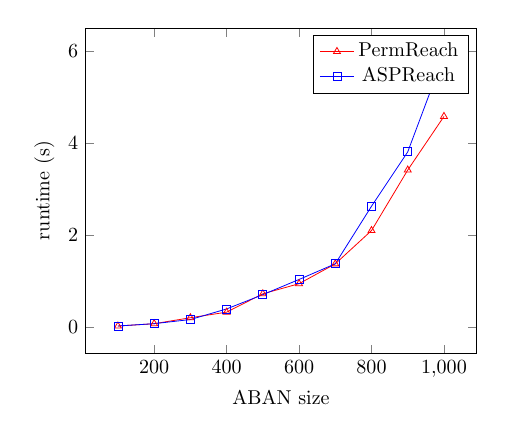
\begin{tikzpicture}[scale=0.725]
    \begin{axis}[xlabel=ABAN size,ylabel=runtime (s)]
       \addplot[mark=triangle,color=red] coordinates{
        (100,0.029)
        (200,0.079)
        (300,0.209)
        (400,0.330)
        (500,0.729)
        (600,0.948)
        (700,1.379)
        (800,2.102)
        (900,3.416)
        (1000,4.58)
        };
        \addlegendentry{PermReach}
       \addplot[mark=square,color=blue] coordinates{
        (100,0.03)
        (200,0.08)
        (300,0.17)
        (400,0.40)
        (500,0.71)
        (600,1.04)
        (700,1.38)
        (800,2.63)
        (900,3.81)
        (1000,5.91)       
        };
        \addlegendentry{ASPReach}
    \end{axis}
\end{tikzpicture}
    \label{fig:sizeTest}
    }
    \subfigure[0.5\linewidth][Runtime with fixing the number of automata to $20$]{
    \centering
    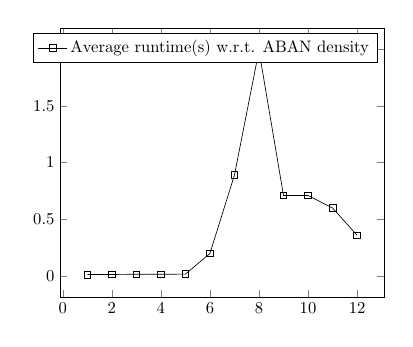
\begin{tikzpicture}[>=stealth,scale=0.6,line width=0.8pt,align=center]
    \begin{axis}%[legend pos=north west]
       \addplot[mark=square] coordinates{
(1,0.014)
(2,0.015)
(3,0.017)
(4,0.017)
(5,0.018)
(6,0.2)
(7,0.89)
(8,1.987)
(9,0.710)
(10,0.71)
(11,0.6)
(12,0.36)    
        %(1,3.57/400)
        %(2,3.9/400)
        %(3,10.4/400)
        %(4,29.4/400)
        %(5,205/400)
        %(6,275/400)
        %(7,1265/400)
        };
        \addlegendentry{Average runtime(s) w.r.t. ABAN density}
    \end{axis}
\end{tikzpicture}

    \label{fig:inconcTest}
    }
    \caption[Runtime tests of reachability analyzers]{Average Runtime tests of PermReach and ASPReach on random generated ABANs}
\end{figure}

\section{Implementation of CRAC and M2RIT}
CRAC and M2RIT are algorithms for revising existing models using reachability information and sets of revisable candidate transitions, with the former adding and removing transitions and the latter revising existing transitions.\footnote{Code and testing data available at \url{https://github.com/XinweiChai/reach_and_revision}}.
We suppose that the sets come from time-series data.

\subsection{CRAC}
CRAC is based on the hypothesis that time-series data is consistent with differential equations.
We test it by the following steps:
\begin{enumerate}
    \item Generate random differential equations $E$
    \item Generate time-series data $tsd$ from $E$
    \item Construct an ABAN $A=(\Sigma, T)$ consistent with $E$, compute its reachability information $Re$, $Un$ using ASPReach
    \item Obtain a partial ABAN $A'=(\Sigma, T')$ with $T'\subset T$, compute its reachability information $Re'$ and $Un'$ using ASPReach
    \item Infer candidate regulations $R$ from $E$
    \item Construct an ABAN $A''=(\Sigma, T')$ based on $A'$, $Re$, $Un$, $Re'$, $Un'$ and $R$ s.t. $A''$ satisfies $Re$, $Un$ using CRAC
\end{enumerate}


In step 1, given the set of variables $\Sigma$, every differential equation associated to $x_v\in \Sigma$ is $\Delta x_v=\sum_{u\in \Sigma'}x_u k_{uv}$. 
To generate such equation, we generate first $\Sigma'\subseteq \Sigma\miset{v}$ randomly.
The first element of $\Sigma'$ is randomly chosen from $\Sigma\miset{v}$.
For $i>1$, if $(i-1)$-th element of $\Sigma'$ exists, we generate the $i$-th element with an 80\% probability, choosing from $\Sigma\setminus(\Sigma'\addset{v})$.
For parameter $k_{uv}$, we choose a random number in $[-1,-0.5]\cup[0.5,1]$.
%Through a rough discretization, we obtain an ABAN from the random differential equations:

In step 2, we generate a possible time-series.
To make it consistent with differential equations (simultaneous change), we choose the next state from synchronous successors.
Every state change can be regarded as a composition of several asynchronous state changes without considering the orders.
One of the drawbacks is that time is not taken into account.

We then hide randomly a part of transitions (20\% of all the transitions) to obtain $T'$. %calculate the percentage of retrieval by CRAC and see even if the resulted transitions are different, whether they can reproduce the time-series data.

From the running result, we discovered that CRAC is not able to retrieve all the transitions in $T$ but can satisfy the reachability properties provided by $A$.
We noticed that the added transitions can be similar to the hidden transitions but with different logic operators, \textit{e.g.} \ac{b_1,c_1}{a_0}{a_1} could be replaced by \ac{b_1}{a_0}{a_1} and \ac{c_1}{a_0}{a_1}.

The performance of CRAC also depends on the discretization  which can be a possible future topic of studies.

%Generate all the reachability instances, test how many CRAC/M2RIT need to retrieve all the missing transitions.

\subsection{M2RIT}
The test of M2RIT is analogous:
\begin{enumerate}
    \item Generate random time-series data $tsd$
    \item Obtain partial time-series data $tsd'\subset tsd$
    \item Infer ABAN $A=(\Sigma, T)$ from $tsd$ using asynchronous LFIT, compute its reachability information $Re$ and $Un$ using ASPReach
    \item Infer ABAN $A'=(\Sigma, T')$ from $tsd'$ using asynchronous LFIT, compute its reachability information $Re'$ and $Un'$ using ASPReach
    \item Construct an ABAN $A''=(\Sigma, T')$ based on $A'$, $Re$, $Un$, $Re'$, $Un'$ s.t. $A''$ satisfies $Re$, $Un$ using M2RIT
\end{enumerate}
We generate a random ABAN like in Section~\ref{sec:compReachAnalyzers}.
We then choose the next state from asynchronous successors are generated by an equi-probable next state.
This operation allows us to obtain a time-series data matching perfectly asynchronous update scheme as there is at most one state change for all automata at each time point. 
Hence, such time-series data fit perfectly asynchronous LFIT algorithm.
However, they do not exist in real world as we cannot limit the number of state changes at each observation.

$$A=\kbordermatrix{\mbox{\footnotesize$t$}&0&1&2&3\\
a&\mathbf{0}&\mathbf{1}&1&1\\
b&\mathbf{0}&\mathbf{1}&0&1\\
c&\mathbf{1}&\mathbf{0}&1&1\\
d&\mathbf{0}&\mathbf{0}&0&1
}
\hspace{2cm}
A'=\kbordermatrix{\mbox{\footnotesize$t$}&0&1&2&3\\
a&\mathbf{0}&\mathbf{1}&1&1\\
b&0&\mathbf{0}&\mathbf{1}&1\\
c&1&1&\mathbf{1}&\mathbf{0}\\
d&0&0&0&0
}
$$
The left matrix $A$ is an example of generalized time series data, where at each time point multiple variables can change their values.
The right matrix $A'$ is an example of ``asynchronous'' time-series data, where at each time point at most one variable changes its value.
From $t=0$ to $t=1$, $A$ shows a direct transition $(0,0,1,0)\to (1,1,0,0)$ where $A'$ interprets this transition in details (from $t=0$ to $t=3$) under the hypothesis that two variables cannot change their values exactly at the same time.

Both can be used as input for CRAC but only the latter one is proper for M2RIT to fit asynchronous LFIT algorithm.

Like in the last section, we hide 20\% of the transitions and offer a set of reachability information.

From the running result, we discover that M2RIT is not able to retrieve all the transitions in $T$ but can construct a new ABAN $A''$ which simulates $A$ in the meaning of reachability.
This behavior resembles that of LFIT algorithm, as it aims at obtaining a model that reproduces the time series data without considering if the model is identical to the real one. 

Limited by the computing capacity of ASPReach, CRAC and M2RIT can deal with models with up to 1000 variables.

\section{R\'esum\'e}

In this chapter, we have shown the performance of the practical implementation of the algorithm introduced in this thesis.
Different results approved the properties of different methodologies shown in the previous chapters.

PermReach and ASPReach show that they are more conclusive than Pint, the former work of our laboratory according to conclusiveness tests.
They are also more efficient than traditional reachability analyzers like Mole and NuSMV according to computing power tests.
Between PermReach and of ASPReach, there is a trade-off between conclusiveness and efficiency: 
PermReach is more efficient than ASPReach but with less conclusiveness.

The tests of CRAC and M2RIT show that they can be applied to revise models with up to $1000$ variables if proper and sufficient reachability information is given.
Unfortunately, there is no existing work that uses reachability properties to revise models, we cannot run a competition between CRAC and M2RIT and the state-of-the-art methods.
